% Copyright 2021 Joel Feldman, Andrew Rechnitzer and Elyse Yeager, except where noted.
% This work is licensed under a Creative Commons Attribution-NonCommercial-ShareAlike 4.0 International License.
% https://creativecommons.org/licenses/by-nc-sa/4.0/


%----------------------------------------------------------------------------------------
\section*{2.8: Derivatives of Trig Functions}

 \begin{frame}{Table of Contents \only<beamer>{\hfill\hyperlink{derivofsine}{\beamerskipbutton{skip trig review}}}}
\mapofcontentsBB{\bi}
 \end{frame}
 \note{Students often feel stressed because they don't know which facts from trigonometry class they are responsible for. So, we start with a quick overview -- less to teach these things than to list what they are responsible for knowing}
%----------------------------------------------------------------------------------------
\begin{frame}[t]
\begin{block}{Basic Trig Functions}
\begin{center}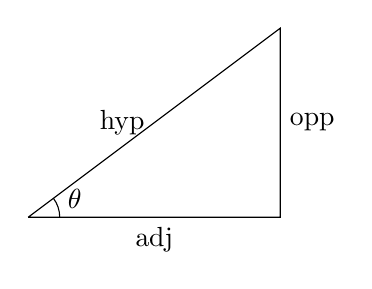
\begin{tikzpicture}[scale=0.8]
\draw (.5,0) arc (0:37:5mm)node[midway,right,yshift=1mm]{$\theta$};
\draw (0,0)--(4,0)node[midway,below]{adj}--(4,3)node[midway,right]{opp}--(0,0)node[midway,left]{hyp};;;
\end{tikzpicture}\end{center}
\begin{multicols}{2}
$\sin(\theta) = \dfrac{\text{opp}}{\text{hyp}}$\\[1mm]
$\cos(\theta) = \dfrac{\text{adj}}{\text{hyp}}$\\[1mm]
$\tan(\theta) = \dfrac{\text{opp}}{\text{adj}}$\\[1mm]
$\csc(\theta) = \dfrac{1}{\sin(\theta)}$\\[1mm]
$\sec(\theta) = \dfrac{1}{\cos(\theta)}$\\[1mm]
$\cot(\theta) = \dfrac{1}{\tan(\theta)}$\\~
\end{multicols}
\end{block}

%draw picture of sin, talk about its derivative
\end{frame}
%-------------------------------------------------------------
\begin{frame}{Commonly used facts}
\begin{itemize}
\item Graphs of sine, cosine, tangent \pause\vfill
\item Sine, cosine, and tangent of reference angles: $0$, $\dfrac{\pi}{6}$, $\dfrac{\pi}{4}$,
$\dfrac{\pi}{3}$, $\dfrac{\pi}{2}$\pause\vfill
\item How to use reference angles to find sine, cosine and tangent of other angles\pause\vfill
\item Identities: $\sin^2 x + \cos ^2 x =1$;
\qquad $\tan^2x+1=\sec^2x$;
\\$\sin^2 x = \dfrac{1-\cos(2x)}{2}$; \qquad
$\cos^2 x = \dfrac{1+\cos 2x}{2}$\pause\vfill
\item Conversion between radians and degrees
\end{itemize}\vfill
CLP-1 has an appendix on high school trigonometry that you should be familiar with.
\end{frame}
%-------------------------------------------------------------
%-------------------------------------------------------------
\begin{frame}{Reference Angles}
\begin{center}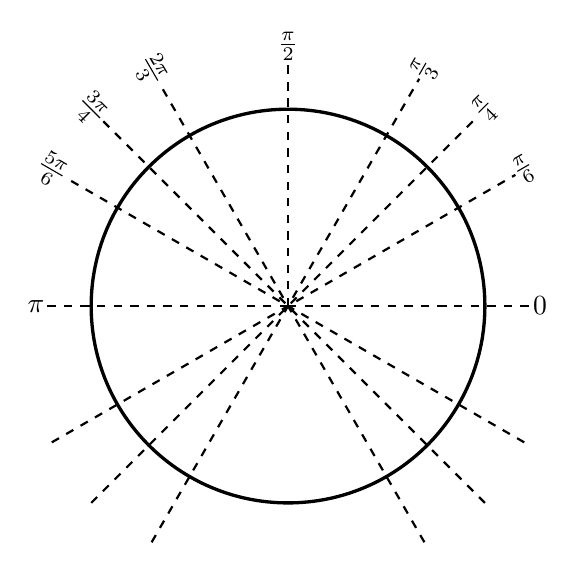
\begin{tikzpicture}[]
\draw[very thick] node[shape=circle, minimum size=5cm, draw]{};
\draw[thick, dashed] plot[domain=0:3.2] (\x,0)
node[fill=white,inner sep=0]{$0$};
\draw[thick, dashed] plot[domain=0:-3.2] (\x,0)
node[fill=white,inner sep=0]{$\pi$};
\draw[thick, dashed] plot[domain=0:3.3] (0,\x)
node[fill=white,inner sep=1.5]{$\frac{\pi}{2}$};
\foreach \pr/\r/\d/\t/\tt in 
{\frac{3\pi}{4}/\frac{\pi}{4}/45/1/2.5,
\frac{2\pi}{3}/\frac{\pi}{3}/60/1.732/1.732,
\frac{5\pi}{6}/\frac{\pi}{6}/30/0.577/3}{
\draw[thick, dashed] plot[domain=-\tt:\tt] (\x,{\t*\x}) node[rotate=\d,fill=white,inner sep=0]{$\r$};
\draw[thick, dashed] plot[domain=-\tt:\tt] (-\x,{\t*\x}) node[rotate=-\d,fill=white,inner sep=0]{$\pr$};
}
\end{tikzpicture}\end{center}
\end{frame}
%-------------------------------------------------------------
%----------------------------------------------------------------------------------------
\begin{frame}[t]{Derivative of Sine \only<beamer>{\hfill\hyperlink{trigderivs}{\beamerskipbutton{skip proofs of sine and cosine derivatives}}}}\label{derivofsine}
\begin{center}
\begin{tikzpicture}
\draw[<->, help lines] (-5,0)--(5,0) node[right]{$x$};
\draw[<->, help lines] (0,-1)--(0,1) node[above]{$y$};
\draw[C2, ultra thick] plot[ domain=-5:5, samples=100] (\x,{sin(\x r)}) node[below]{$y=\sin(x)$};
\onslide<3-4|handout:0>{\draw[M4, ultra thick, ->] (1.6,-.5)--(1.6,-.2);}
\onslide<4-|handout:0>{\draw (1.6,0) node[vertex, M4]{};}
\onslide<5-6|handout:0>{\draw[M4, ultra thick, ->] (-1.6,-.5)--(-1.6,-.2);
\draw[M4, ultra thick, ->] (-4.7,-.5)--(-4.7,-.2);
\draw[M4, ultra thick, ->] (4.7,-.5)--(4.7,-.2);}
\onslide<6-|handout:0>{\draw (-1.6,0) node[vertex, M4]{};
\draw (-4.7,0) node[vertex, M4]{};
\draw (4.7,0) node[vertex, M4]{};}
\onslide<7-8|handout:0>{\draw[ultra thick, M4, <->] (-1.6,-.5)--(1.6,-.5);}
\onslide<8-|handout:0>{\draw[ultra thick, M4] plot[domain=-1.6:1.6, samples=100](\x,{cos(\x r)});}
\onslide<9|handout:0>{\draw[ultra thick, M4, <->] (1.6,-.5)--(4.7,-.5);
\draw[ultra thick, M4, <->] (-4.7,-.5)--(-1.6,-.5);}
\onslide<10-|handout:0>{\draw[ultra thick, M4] plot[domain=-4.7:1.6, samples=100](\x,{cos(\x r)});
\draw[ultra thick, M4] plot[domain=1.6:4.7](\x,{cos(\x r)}); }
\end{tikzpicture}
\end{center}

\onslide<2->{\color{M4}Consider the derivative of $f(x)=\sin(x)$.}
\note<11>{By plotting points we know (easy to find where deriv is zero; then where it's positive/negative/max) it seems \textit{likely} that the deriv of sine is cosine. But this isn't a proof. Nice to mention that when we're using degrees instead of radians, the deriv of sine is NOT cosine. Proof follows but it's basically a TED talk -- you won't be assessed on it.}
\onslide<11-|handout:0>{\[\diff{}{x}\{\sin(x)\}\stackrel{?}{=}\cos(x).\]}
\end{frame}
%----------------------------------------------------------------------------------------

%----------------------------------------------------------------------------------------
\begin{frame}[t]\small
%\hfill\smash{\only<beamer>{\hfill\hyperlink{trigderivs}{\beamerskipbutton{skip proofs of sine and cosine derivatives}}}}\\
$\diff{}{x}\{\sin x\} = \displaystyle\lim_{h \rightarrow 0 } \frac{\alert<2>{\sin(x+h)}-\sin(x)}{h}$\ \pause\vfill
$=\displaystyle\lim_{h \rightarrow 0 } \dfrac{\alert<2>{\sin(x)\cos(h)+\cos(x)\sin(h)}-\sin(x)}{h}$\pause \vfill

%$=\displaystyle\lim_{h \rightarrow 0} 
%\dfrac{\sin(x)(\cos(h)-1)+\cos(x)\sin(h)}{h}$\pause\vfill

$=\displaystyle\lim_{h \rightarrow 0} 
\dfrac{\sin(x)(\cos(h)-1)}{h}
+\displaystyle\lim_{h \rightarrow 0} \dfrac{\cos(x)\sin(h)}{h}$\pause\vfill

%$=\sin (x)\alert<6>{ \displaystyle\lim_{h \rightarrow 0}
%\dfrac{\cos(h)-1}{h}} + \cos(x)\displaystyle\lim_{h \rightarrow 0 }\dfrac{\sin(h)}{h}$\pause\vfill

$=\sin (x) \textcolor{M4}{\displaystyle\lim_{h \rightarrow 0}
\dfrac{\cos(0+h)-\cos(0)}{h}} + \cos(x)
\textcolor{M3}{\displaystyle\lim_{h \rightarrow 0 }\dfrac{\sin(h)}{h}}$\pause\vfill

$=\sin(x)\textcolor{M4}{\left.\diff{}{x}\{\cos(x)\}\right\vert_{x=0}} +
\cos(x)
\textcolor{M3}{\displaystyle\lim_{h \rightarrow 0 }\dfrac{\sin(h)}{h}}$ \pause \hfill $=$ \hfill
\framebox{$\cos(x)\textcolor{M3}{\displaystyle\lim_{h \rightarrow 0} \frac{\sin(h)}{h}}$}

\vfill
since $\cos(x)$ has a horizontal tangent, and hence has derivative zero, at $x=0$. 
\end{frame}
%----------------------------------------------------------------------------------------
\note{Now, the question becomes: what is that limit? Once again, it's important to note that we are measuring in radians, not degrees.}
%----------------------------------------------------------------------------------------
\begin{frame}<beamer>
\StatusBar{2}{7}
\only<1>{First, we investigate $\lim\limits_{h \to 0}\frac{\sin h}{h}$ informally.}\pause
\begin{center}
	\begin{tikzpicture}
	\clip(-1,-1) rectangle (9,8);
	\draw (0,0)node[shape=circle, minimum size=16cm,draw]{};
	\draw (-8,0)--(9,0) (0,-8)--(0,9);
	\onslide<1-2>{
		\draw[thick] (0,0)--(5.66,5.66);
		\draw[thick] (1,0) arc (0:45:1cm)node[midway,right]{$x$};}
	\onslide<2>{	\draw[ultra thick,C4](5.66,5.66)--(5.66,0)node[midway, left]{$\sin h$};
		\draw[ultra thick,M4,|-|] (8,0) arc (0:45:8cm)node[midway, right]{$h$};}
	
	\foreach \n in {1,...,7}{
		\ADD{\n}{2}{\s}%s: slide
		\onslide<\s>{	\MULTIPLY{\n}{5}{\m}
			\SUBTRACT{45}{\m}{\x} %x: angle in degrees
			\MULTIPLY{\x}{3.14159}{\px}
			\DIVIDE{\px}{180}{\r}%r: angle in radians
			\SIN{\r}{\sr} %sr: sin(r)
			\MULTIPLY{\sr}{8}{\y}
			\COS{\r}{\cr}%cr: cosr
			\MULTIPLY{\cr}{8}{\xlength}
			\draw[thick] (0,0)--(\xlength,\y);
			
			\draw[thick] (1,0) arc (0:\x:1cm)node[midway, right]{$x$};;
			\draw[ultra thick,C4] (\xlength,\y)--(\xlength,0)node[midway, left]{$\sin h$};
			\draw[ultra thick, M4,|-|] (8,0) arc (0:\x:8cm)node[midway, right]{$h$};
	}}

	\end{tikzpicture}
\end{center}

\end{frame}
%----------------------------------------------------------------------------------------
\begin{frame}<beamer>[t]
It seems $\sin h \approx h$ when $h \approx 0$, so $\lim\limits_{h \to 0}\frac{\sin h}{h}\stackrel{?}{=}1$.

\vspace{1cm}

We can prove this more formally using the Squeeze Theorem and more trigonometry.
We will first prove that $\frac{\sin(h)}{h}\le 1$ and then we will prove that
$\frac{\sin(h)}{h}\ge\cos(h)$. Then we will apply the Squeeze Theorem.

\vspace{1cm}

Here is the proof that $\frac{\sin(h)}{h}\le 1$.
\end{frame}
%----------------------------------------------------------------------------------------
\begin{frame}[t]
\StatusBar{1}{14}
\only<-14>{\begin{center}
\begin{tikzpicture}[scale=4]

%\draw (-.5,.5) node{$\onslide<14-16|handout:0>{\cos h \leq}\dfrac{\sin h}{h}\onslide<4-16>{\leq 1}$};

\clip (-.25,-.25) rectangle (1.5,1.1);

\draw[help lines] (-1.1,0)--(1.1,0) (0,-1.1)--(0,1.1);
\draw (0,0) circle (1cm);

\draw (0,0)--(.7,.7);
\draw (.3,.37) node[rotate=45]{$1$};
\draw[M4, ultra thick] (.7,.7)--(.7,0);
\draw (.2,.075) node{\textcolor{W4}{$h$}};
\draw (.625,.3) node[rotate=90]{\textcolor{M4}{$\sin(h)$}};

%\onslide<handout:0>{
\onslide<2-4>{
\draw[W4, ultra thick] (1,0) arc (0:45:1cm);
\draw (0.95,.45) node{\textcolor{W4}{$h$}};
}

\onslide<5->{
\draw (.7,.7)--(1,1);
\draw[C2, ultra thick](1,1)--(1,0);
\onslide<6->{\draw[C2] (1.1,.3) node[rotate=90]{$\tan(h)$};}}

\onslide<7,9-10,13-|handout:0>{
\draw[W4, fill, opacity=.1] (0,0)--(1,0) arc (0:45:1cm)--(0,0);
}

\onslide<8,11-|handout:0>{
\draw[C2, fill, opacity=.1] (0,0)--(1,0)--(1,1)--(0,0);
}
%}
\end{tikzpicture}
\end{center}}

\onslide<handout:0>{\only<3-15>{
\onslide<3-4>{ \textcolor{M4}{$\sin(h)$}$\leq$\textcolor{W4}{$h$} 
\onslide<4>{ so \framebox{$\dfrac{\sin(h)}{h} \leq 1$}}}
\onslide<4>{\linebreak Now for the proof  that $\dfrac{\sin(h)}{h} \geq \cos(h)$.}

\vspace{-2cm}
\onslide<9-14>{\textcolor{W4}{green area:\onslide<10-14>{ $ \dfrac{h}{2}$}}}
\hfill
\onslide<13-14>{$\textcolor{W4}{\dfrac{h}{2}}\leq \textcolor{C2}{\dfrac{\tan(h)}{2}}$}
\hfill
\onslide<11-14>{\textcolor{C2}{Blue area: \onslide<12-14>{$\dfrac{\tan h}{2}$}}}

\onslide<14-14>{ \[\boxed{\cos(h) \leq \dfrac{\sin(h)}{h}}\]}}

\only<15->{%\vspace{-5mm}
We are now ready for the Squeeze Theorem. We have
\begin{align*}
&\cos h &&\leq&& \frac{\sin h}{h}&&\leq&&1\\
\onslide<16->{\lim_{h \to 0}&\cos h =1&&&&&&& \lim_{h \to 0}&1=1}
\onslide<17->{\intertext{By the Squeeze Theorem,}}
\onslide<18->{&&&&\color{M4}\lim_{h \to 0}&\color{M4}\frac{\sin h}{h}=1}
\end{align*}
}
}
\unote{Lemma~\eref{text}{lem sinhoverh}}
\end{frame}

%-------------------------------------------------------------
\begin{frame}[t]{Derivatives of Sine and Cosine}
>From before,
\[\alert<2->{\diff{}{x}\{\sin(x)\}} = \cos(x)\cdot \lim_{h \rightarrow 0 }\frac{\sin(h)}{h} = \onslide<2->{\alert<2->{\cos(x)}}\]

%\only<3-8>{\begin{center}
%\begin{tikzpicture}[scale=0.9]
%\myaxis{}{5}{5}{}{1}{1}
%\onslide<3>{\draw[thick, M4] plot[domain=-5:5, samples=100](\x,{sin (2*\x r)}) node[right]{$y=\sin x$};}
%\onslide<4->{\draw[thick, M4!50] plot[domain=-5:5, samples=100](\x,{sin (2*\x r)}) node[right]{$y=\sin x$};}
%
%\onslide<4>{\draw[thick, C2] plot[domain=-5:4.6, samples=100](\x,{cos (2*\x r)}) node[right]{$y=\cos x$};
%\draw[C2!50!M4, very thick, ->] (0.8,1.2)--(0,1.2);}
%\onslide<5>{\draw[thick, C2!50] plot[domain=-5:4.6, samples=100](\x,{cos (2*\x r)}) node[right]{$y=\cos x$};
%\draw[C2!30!M4!30, very thick, ->] (0.8,1.2)--(0,1.2);}
%
%\onslide<5-6>{\draw[thick, C4] plot[domain=-5:5, samples=100](\x,{-sin (2*\x r)});
%\draw[C2!50!C4, very thick, ->] (0,1.2)--(-0.8,1.2);}
%\onslide<7->{\draw[thick, C4] plot[domain=-5:5, samples=100](\x,{-sin (2*\x r)}) node[right]{$y=-\sin x$};
%\draw[C2!50!C4, very thick, ->] (0,1.2)--(-0.8,1.2);}
%\end{tikzpicture}
%\end{center}
%\onslide<8-|handout:0>{We might reasonably expect: \qquad
%$\diff{}{x}\{\cos x\}=-\sin x$.}}

%\onslide<9-|handout:0>{
%\begin{align*}
%{\diff{}{x}\{\cos(x)\}}&=\lim_{h \rightarrow 0 }\frac{\cos(x+h)-\cos(x)}{h}\\
%\onslide<10->{&=\lim_{h \rightarrow 0 }\frac{\cos(x)\cos(h)-\sin(x)\sin(h)-\cos(x)}{h}\\
%&=\cos(x)\lim_{h \rightarrow 0 }\frac{\cos(h)-1}{h}
%-
%\sin(x)\lim_{h \rightarrow 0 }\frac{\sin(h)}{h}\\
%&=\cos(x)(0) - \sin(x)(1) ={ -\sin(x)}}
%\end{align*}
%}
\end{frame}
%-------------------------------------------------------

\begin{frame}[t]{Derivative of Cosine}
Now for the derivative of $\cos$. We already know the derivative of $\sin$,
and it is easy to convert between $\sin$ and $\cos$ using trig identities.
\begin{multicols}{2}
	\begin{tikzpicture}[scale=0.9]
	\draw (0,0)-|(4,3)--cycle;
	\draw (0,0)--(4,0)node[midway,below]{a}--(4,3)node[midway,right]{b}--(0,0)node[midway,left]{c};
	\draw (.5,0) arc (0:37:.5cm)node[midway, right,yshift=1mm]{$x$};
		\color{M4}
		\onslide<2|handout:0>{\draw (4,2.5) arc(270:217:.5cm)node[midway, below]{$\theta$};}
		\onslide<3->{\draw (4,2) arc(270:217:1cm)node[midway,below,xshift=-.25cm ]{$\frac{\pi}{2}-x$};}
		\color{black}
	\end{tikzpicture}
	
	\onslide<4->{\begin{align*}
				\sin x &= \frac{b}{c}=\cos\left(\frac{\pi}{2}-x\right)\\
				\cos x &= \frac{a}{c}=\sin\left(\frac{\pi}{2}-x\right)\\
			\end{align*}}
\end{multicols}
	
	\onslide<5-|handout:0>{\small\color{answercolor}{ $\diff{}{x}\left[\cos(x) \right]
   =\diff{}{x}\left[\sin\left(\frac{\pi}{2}-x \right) \right]
   =-\diff{}{x}\left[\sin\left(x-\frac{\pi}{2}\right) \right]
   =-\cos\left(x-\frac{\pi}{2}\right)=\color{M4}-\sin x$}
				
\vspace{0.5cm}
\color{black}{since $\sin(-\theta)=-\sin(\theta)$ and $\cos(-\theta)=\cos(\theta)$.}}


\StatusBar{1}{5}

\end{frame}
%----------------------------------------------------------------------------------------
%\begin{frame}[t]{Derivatives of Sine and Cosine}
%From before,
%\[\alert<2->{\diff{}{x}\{\sin(x)\}} = \cos(x)\cdot \lim_{h \rightarrow 0 }\frac{\sin(h)}{h} = \onslide<2->{\alert<2->{\cos(x)}}\]
%
%\only<3-8>{\begin{center}
%\begin{tikzpicture}[scale=0.9]
%\myaxis{}{5}{5}{}{1}{1}
%\onslide<3>{\draw[thick, M4] plot[domain=-5:5, samples=100](\x,{sin (2*\x r)}) node[right]{$y=\sin x$};}
%\onslide<4->{\draw[thick, M4!50] plot[domain=-5:5, samples=100](\x,{sin (2*\x r)}) node[right]{$y=\sin x$};}
%
%\onslide<4>{\draw[thick, C2] plot[domain=-5:4.6, samples=100](\x,{cos (2*\x r)}) node[right]{$y=\cos x$};
%\draw[C2!50!M4, very thick, ->] (0.8,1.2)--(0,1.2);}
%\onslide<5>{\draw[thick, C2!50] plot[domain=-5:4.6, samples=100](\x,{cos (2*\x r)}) node[right]{$y=\cos x$};
%\draw[C2!30!M4!30, very thick, ->] (0.8,1.2)--(0,1.2);}
%
%\onslide<5-6>{\draw[thick, C4] plot[domain=-5:5, samples=100](\x,{-sin (2*\x r)});
%\draw[C2!50!C4, very thick, ->] (0,1.2)--(-0.8,1.2);}
%\onslide<7->{\draw[thick, C4] plot[domain=-5:5, samples=100](\x,{-sin (2*\x r)}) node[right]{$y=-\sin x$};
%\draw[C2!50!C4, very thick, ->] (0,1.2)--(-0.8,1.2);}
%\end{tikzpicture}
%\end{center}
%\onslide<8-|handout:0>{We might reasonably expect: \qquad
%$\diff{}{x}\{\cos x\}=-\sin x$.}}
%
%\onslide<9-|handout:0>{
%\begin{align*}
%{\diff{}{x}\{\cos(x)\}}&=\lim_{h \rightarrow 0 }\frac{\cos(x+h)-\cos(x)}{h}\\
%\onslide<10->{&=\lim_{h \rightarrow 0 }\frac{\cos(x)\cos(h)-\sin(x)\sin(h)-\cos(x)}{h}\\
%&=\cos(x)\lim_{h \rightarrow 0 }\frac{\cos(h)-1}{h}
%-
%\sin(x)\lim_{h \rightarrow 0 }\frac{\sin(h)}{h}\\
%&=\cos(x)(0) - \sin(x)(1) ={ -\sin(x)}}
%\end{align*}
%}
%\end{frame}
%-------------------------------------------------------
%----------------------------------------------------------------------------------------
\begin{frame}[t]\label{trigderivs}
When we use radians:
\begin{block}{Derivatives of Trig Functions}
\begin{multicols}{2}
\indent\alert{$\diff{}{x}\{\sin(x)\}=\cos(x)$\\
$\diff{}{x}\{\cos(x)\}=-\sin(x)$}\\
$\diff{}{x}\{\tan(x)\}=$\\

$\diff{}{x}\{\sec(x)\}=$\\
$\diff{}{x}\{\csc(x)\}=$\\
$\diff{}{x}\{\cot(x)\}=$\\~
\end{multicols}
\end{block}

\begin{block}{Honorable Mention}
\[\alert{\lim_{x \rightarrow 0 }\frac{\sin x}{x} = 1}\]
\end{block}

\unote{Lemma~\eref{text}{lem DIFFsincos}}
\end{frame}
%----------------------------------------------------------------------------------------
\begin{frame}\centering
\note{Remember, these are only true using radians.}
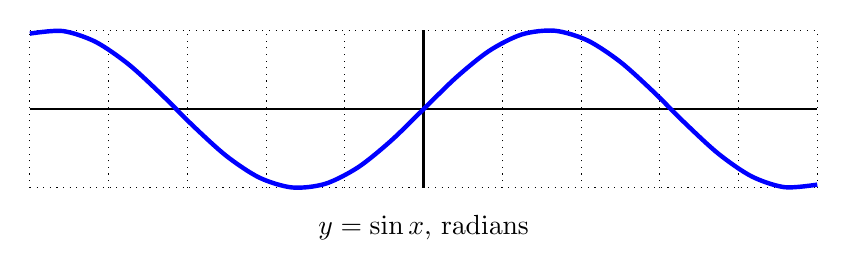
\begin{tikzpicture}
\draw[dotted] (-5,-1) grid (5,1);
\draw[thick] (-5,0)--(5,0) (0,-1)--(0,1);
\draw[ultra thick, blue] plot[domain=-5:5,smooth](\x,{sin(\x r)});
\draw (0,-1.5)node{$y=\sin x$, radians};
\xcoord{1}{1} \ycoord{1}{1}
\end{tikzpicture}
\vfill
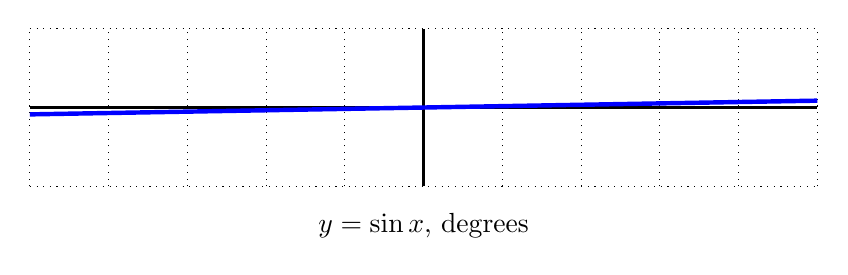
\begin{tikzpicture}
\draw[dotted] (-5,-1) grid (5,1);
\draw[thick] (-5,0)--(5,0) (0,-1)--(0,1);
\draw[ultra thick, blue] plot[domain=-5:5,smooth](\x,{sin(\x)});
\draw (0,-1.5)node{$y=\sin x$, degrees};
\xcoord{1}{1} \ycoord{1}{1}
\end{tikzpicture}

\end{frame}
%----------------------------------------------------------------------------------------
%----------------------------------------------------------------------------------------
\note{Can go through tangent, but no need to do the rest. Just make sure students know how they could be computed from sines and cosines, should they so desire}
%----------------------------------------------------------------------------------------
\begin{frame}[t]{Other Trig Functions  \only<beamer>{\hfill\hyperlink{alltrigderivs}{\beamerskipbutton{skip proofs of other trig derivatives}}}}
\AnswerSpace\only<1>{\AnswerYes}

\[\tan(x)=\frac{\sin(x)}{\cos(x)}\]\vfill\pause

\answer{
\begin{align*}
\alert{\diff{}{x}[\tan(x)]} &= \ds\diff{}{x}\left[ \dfrac{\sin(x)}{\cos(x)}\right]\\
&=\dfrac{\cos(x)\cos(x)-\sin(x)[-\sin(x)]}{\cos^2(x)}\\ 
&=\dfrac{\cos^2(x)+\sin^2(x)}{\cos^2(x)}\\ 
&=\dfrac{1}{\cos^2(x)} = \alert{\sec^2(x)}
\end{align*}}
\end{frame}

%----------------------------------------------------------------------------------------
\begin{frame}[t]{Other Trig Functions  \only<beamer>{\hfill\hyperlink{alltrigderivs}{\beamerskipbutton{skip proofs of other trig derivatives}}}}
\AnswerSpace\only<1>{\AnswerYes}

\[\sec(x)=\frac{1}{\cos(x)}\]\vfill\pause

\begin{align*}
\alert{\diff{}{x}[\sec(x)]} &= \ds\diff{}{x}\left[ \dfrac{1}{\cos(x)}\right]\\
&=\dfrac{\cos(x)(0)-(1)(-\sin(x))}{\cos^2(x)}\\
&=\dfrac{\sin(x)}{\cos^2(x)}\\
&=\dfrac{1}{\cos(x)}\dfrac{\sin(x)}{\cos(x)}\\
&= \alert{\sec(x)\tan(x)}
\end{align*}
\end{frame}
%----------------------------------------------------------------------------------------
\begin{frame}[t]{Other Trig Functions  \only<beamer>{\hfill\hyperlink{alltrigderivs}{\beamerskipbutton{skip proofs of other trig derivatives}}}}
\AnswerSpace\only<1>{\AnswerYes}

\[\csc(x)=\frac{1}{\sin(x)}\]\vfill\pause

\begin{align*}
\alert{\diff{}{x}[\csc(x)]} &= \ds\diff{}{x}\left[ \dfrac{1}{\sin(x)}\right]\\
&=\dfrac{\sin(x)(0)-(1)\cos(x)}{\sin^2(x)}\\
&=\dfrac{-\cos(x)}{\sin^2(x)}\\
&=\dfrac{-1}{\sin(x)}\dfrac{\cos(x)}{\sin(x)}\\
&= \alert{-\csc(x)\cot(x)}
\end{align*}
\end{frame}

%----------------------------------------------------------------------------------------
\begin{frame}[t]{Other Trig Functions  \only<beamer>{\hfill\hyperlink{alltrigderivs}{\beamerskipbutton{skip proofs of other trig derivatives}}}}
\AnswerSpace\only<1>{\AnswerYes}

\[\cot(x)=\frac{\cos(x)}{\sin(x)}\]\vfill\pause

\begin{align*}
\alert{\diff{}{x}[\cot(x)]} &= \ds\diff{}{x}\left[ \dfrac{\cos(x)}{\sin(x)}\right]\\
&=\dfrac{\sin(x)(-\sin(x))-\cos(x)\cos(x)}{\sin^2(x)}\\
&=\dfrac{-1}{\sin^2(x)}\\
&= \alert{-\csc^2(x)}\end{align*}
\end{frame}
%----------------------------------------------------------------------------------------
\begin{frame}{Memorize}\label{alltrigderivs}

\begin{align*}
\textstyle\diff{}{x}\{\sin(x)\}&=\cos(x)
&\textstyle\diff{}{x}\{\sec(x)\}&=\sec(x)\tan(x)\\
\textstyle\diff{}{x}\{\cos(x)\}&=-\sin(x)
&\textstyle\diff{}{x}\{\csc(x)\}&=-\csc(x)\cot(x)\\
\textstyle\diff{}{x}\{\tan(x)\}&=\sec^2(x)
&\textstyle\diff{}{x}\{\cot(x)\}&=-\csc^2(x)\\[1em]
\lim_{x \rightarrow 0 }\frac{\sin x}{x} &= 1
\end{align*}

\unote{Theorem~\eref{text}{thm:DIFFtrigDerivs}}
\end{frame}
%----------------------------------------------------------------------------------------
\answer{\begin{frame}
\NowYou
\begin{enumerate}
\item Let $f(x)=\dfrac{x\tan(x^2+7)}{15e^x}$. Use the \textbf{definition of the derivative} to find $f'(0)$.\vfill

\item Differentiate $\left(e^x+\cot x\right)\left(5x^6-\csc x\right)$.% (No need to simplify.)\\
%Recall $\diff{}{x}\{\cot x\} = -\csc^2 x$ and $\diff{}{x}\{\csc x\} = -\csc x \cot x$
\vfill

\item  Let $h(x)=\left\{\begin{array}{ccc}
\frac{\sin x}{x}&,& x <0\\
\frac{ax+b}{\cos x}&,&x \ge 0
\end{array}\right.$
\\
Which values of $a$ and $b$ make $h(x)$ continuous at $x=0$?
\end{enumerate}
\MoreSpace\AnswerNo
\end{frame}}
%----------------------------------------------------------------------------------------
\begin{frame}[t]\AnswerNo
\begin{QuestionSet}
\SetQuestion{Let $f(x)=\dfrac{x\tan(x^2+7)}{15e^x}$. Use the {definition of the derivative} to find $f'(0)$.}
\SetQuestion{Differentiate $\left(e^x+\cot x\right)\left(5x^6-\csc x\right)$.}
\SetQuestion{Let $h(x)=\left\{\begin{array}{ccc}
\frac{\sin x}{x}&,& x <0\\
\frac{ax+b}{\cos x}&,&x \ge 0
\end{array}\right.$
\\
Which values of $a$ and $b$ make $h(x)$ continuous at $x=0$?}
\end{QuestionSet}
\end{frame}
%----------------------------------------------------------------------------------------

\begin{frame}
Practice and Review
\note{Not to do in class (unless you have extra time to fill)}
\end{frame}
%----------------------------------------------------------------------------------------
\begin{frame}[t]\AnswerYes
\[f(x)=\left\{\begin{array}{ccc}
x^2\cos\left(\frac{1}{x}\right)&,&x \neq 0\\
0 & , & x=0
\end{array}\right.\]

Is $f(x)$ differentiable at $x=0$?
\vfill
\[g(x)=\left\{\begin{array}{ccc}
e^{\frac{\sin x}{x}}&,&x < 0\\
(x-a)^2 & , & x\ge 0
\end{array}\right.\]

What value(s) of $a$ makes $g(x)$ continuous at $x=0$?

\vfill
\QuestionBar{1}{3}
\end{frame}
%----------------------------------------------------------------------------------------
\begin{frame}<handout:0>[t]
\AnswerBar{1}{3}
\color{answercolor}
We don't have rules for differentiating $f(x)$ at $x=0$, so we have to fall back on the definition of the derivative.
\begin{align*}
f'(0)&=\lim_{h \to 0}\frac{f(h)-f(0)}{h} = \lim_{h\to 0}\frac{h^2\cos\left(\frac1h\right)-0}{h}\\
&= \lim_{h\to 0} h\cos\left(\frac1h\right)=0\\
\end{align*}
Since the limit exists, $f(x)$ is differentiable at 0.
\vfill

\color{C1}
By the definition of continuity, $g(x)$ is continuous at $x=0$ if
\[\lim_{x \to 0}g(x)=g(0)\]
\begin{itemize}\color{answercolor}
\item $g(0)=(0-a)^2=a^2$
\item $\lim\limits_{x \to 0^-}g(x) = \lim\limits_{x \to 0^-}e^{\frac{\sin x}{x}} = e^1=e$
\item $\lim\limits_{x \to 0^+}g(x) = \lim\limits_{x \to 0^+}(x-a)^2 = a^2$
\end{itemize}
In order for $g(x)$ to be continuous, we need $a^2=e$. That is, $a=\sqrt e$ or $a=-\sqrt e$.
\end{frame}
%----------------------------------------------------------------------------------------
\begin{frame}[t]\AnswerSpace
A ladder 3 meters long rests against a vertical wall. Let $\theta$ be the angle between the top of the ladder and the wall, measured in radians, and let $y$ be the height of the top of the ladder. If the ladder slides away from the wall, how fast does $y$ change with respect to $\theta$?

When is the top of the ladder sinking the fastest? The slowest?\vfill

\only<1|handout:1>{
\AnswerYes\QuestionBar{2}{3}
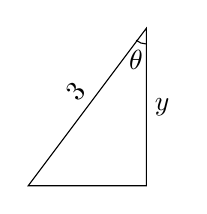
\begin{tikzpicture}
\draw (0,0)--(1.5,0)--(1.5,2)--cycle;
\draw (1.5,1.8) arc (270:230:2mm);
\draw (1.37,1.6) node{$\theta$};
\draw (1.7,1) node{$y$};
\draw (0.6,1.2) node[rotate=50]{$3$};
\end{tikzpicture}\vfill
}

\color{answercolor}
\only<2|handout:0>{\AnswerBar{2}{3}
We want to find how fast $y$ is changing with respect to $\theta$, so we want $\frac{dy}{d\theta}$, or $y'(\theta)$. To calculate that, we need to find $y$ as a function of $\theta$. Note that the ladder forms a right triangle with the wall, and $y$ is the side adjacent to $\theta$, while $3$ is the hypotenuse.
So, $\cos (\theta)=\frac{y}{3}$, hence $y=3\cos(\theta)$. Now we differentiate, and see
\[\frac{dy}{d\theta} = -3\sin(\theta)\]

To answer the other questions, note that $\theta$ never gets larger than $\pi/2$, since at that point the ladder is lying on the ground. When $0 \leq \theta \leq \pi/2$, the smaller $\theta$ gives the smaller rate of change (in absolute value); so the top of the ladder is sinking slowly at first, then faster and faster, fastest just as it hits the ground.}
\end{frame}
%----------------------------------------------------------------------------------------
\begin{frame}[t]\AnswerSpace
Suppose a point in the plane that is $r$ centimetres from the origin, at an angle of $\theta$ ($0 \le \theta \le \frac{\pi}{2}$), is rotated $\pi/2$ radians. What is its new coordinate $(x,y)$? If the point rotates at a constant rate of $a$ radians per second, when is the $x$ coordinate changing fastest and slowest with respect to $\theta$?\vfill


\only<1|handout:1>{\AnswerYes\QuestionBar{3}{3}
\begin{center}
\begin{tikzpicture}
\myaxis{x}{3.5}{3.5}{y}{0}{3.5}
\draw[thick] (0,0)--(3,1) node[midway, above]{$r$};
\draw (3,1) node[vertex, label=right:{$(a,b)$}]{};
\draw (1,.15) node{$\theta$};
\draw (.8,0) arc (0:18.4:.8cm);

\color{M3}
\draw[thick] (0,0)--(-1,3) node[midway, left]{$r$};
\draw (-1,3) node[vertex, label=above:{$(x,y)$}]{};
\draw (.2,1.2) node{$\frac{\pi}{2}$};
\draw[double] (.9,.31) arc (19:109.5:.9cm);

\end{tikzpicture}
\end{center}
}

\color{answercolor}
\only<2|handout:0>{\AnswerBar{3}{3}
\[ x=r\cos\left(\theta+\frac{\pi}{2}\right)=-r\sin(\theta) \]
and 
\[ y=r\sin\left(\theta+\frac{\pi}{2}\right)=r\cos(\theta) \]
To find how fast $x$ is changing with respect to $\theta$,
we take $x'(\theta)=-r\cos(\theta)$. We see that when $\theta=0$, $x$ changes a lot when $\theta$ changes; and when $\theta=\pi/2$, $x$ only changes a little when $\theta$ changes. 
%\vfill
%\href{https://www.siggraph.org/education/materials/HyperGraph/modeling/mod_tran/2drota.htm}{link: explanation of 2d rotation}
}

\end{frame}
%----------------------------------------------------------------------------------------
%\begin{frame}[t]{Practice}
%You have a rope tied to a sled, and you're dragging the sled along the ground. The coefficient of friction is 0.5, and the weight of the sled is 100 pounds. If the angle the rope makes with the sled is $\theta$, then the force you need to exert to move the sled at a constant rate is:
%\[F(\theta) = \frac{50}{\cos(\theta)+.5\sin(\theta)}.\]

%Do you expect $\dfrac{dF}{d\theta}\left(\frac{\pi}{4}\right)$ to be positive or negative?
%What is the rate of change of $F$ with respect to $\theta$?
%\vfill

%\href{http://www.dummies.com/how-to/content/how-to-calculate-work-based-on-force-applied-at-an.html}{Link: Explanation of Pulling an Object at an Angle}
%\end{frame}
%----------------------------------------------------------------------------------------
%----------------------------------------------------------------------------------------
